\documentclass[11pt]{article}
\usepackage[utf8x]{inputenc}
\usepackage[parfill]{parskip}
\usepackage{ucs}
\usepackage[english]{babel}
\usepackage{amsmath}
\usepackage{graphicx}
\usepackage{todonotes}
\usepackage{titlesec}
\usepackage{multirow}
\usepackage{longtable}
\usepackage{cite}
\usepackage{pdfpages}

\begin{document}
\title{Revisiting Minimax play at Wimbledon}
\author{
  Xia, Mengxuan
  \and
  Huang, Kuangxi
}
\date{\today}
\maketitle

\listoftodos

\begin{abstract}

\end{abstract}


\section{Introduction}

In 2001, Walker and Wooders~\cite{walker2001minimax} analyzed the serve choices in Grand Slam tennis matches to provide an empirical study of the mixed strategy equilibrium. Their result indicates no statistical differences in the win rates for male professional tennis players across different strategies. This shows that the experimental result is consistent with the theoretical Minimax play equilibrium. However, they noted that even the best male players had tendency to switch strategies too often to be truly random, resulting in serial dependence. 

Hsu et al.~\cite{hsu2007minimax} contributed in extending Walker et al's empirical analaysis by collecting and studing a broader data set in tennis, inuding male, female and junior matches. They found that there was a mixed evidence in support of of the minimax hypothesis. Although their data pass all the tests in Walker and Wooders, they noted that the serial dependence was a major concern. 

A similar study was conducted on the penalty kicks in Soccer by Chiappori et al~\cite{chiappori2002testing}. They noted that their emperical results on the penalty kicks were consistent to the theoritical mixed-strategy equilibria.
However, they noted that they could not reject that players optimally chose strategies, conditional on the opponent's behavior.

The game of tennis have changed drastically, perhaps more than ever before, over the past decade. With the aid of modern racket and string technology, professional tennis players can now generate tremendous power and spin on their shots in baseline rallies (while the service stroke is not benefited from new technology.) \todo{Do we have citation here? We probably need it} Due to these technological innovations in equipment, the professional players now tend to favor baseline tennis more so than serve and volley tennis of the past, and therefore the importance of the serve as a tennis stroke has been diminished. Also, most if not all professional tennis stadiums have slowed down the bounce speed of their courts, further diminishing the importance of the serve. \todo{citation}

In this paper, we revisit Walker et al's study by collecting a more recent data set to confirm whether the evolution of technologies has an impact on the consistency of minimax play in professional tennis players. Also, players' playing styles vary drastically between surfaces, and therefore service strategy and the overall importance of the serve will vary between surfaces. Thus, it is worth looking into whether the same results hold between the four major surfaces in the modern tennis calendar, namely, grass, clay, outdoor hard-courts and indoor hard-courts.

\section{Replicating the tests}

We begin by explaining how Walker and Wooders' originally modelled the game and collected their data. Our data recording slightly adjusted from their original scheme in order to get data on the sequences of the serves, which will serve the analysis on the sequence of the directions of servers.\todo{Check if I used the right terms here}

\subsection{Modelling the game}
We follow Walker and Wooders to model each serve in a point game by a two-by-two payoff matrix depicted in Table~\ref{table:payoffmatrix}. Let $L$ and $R$ denote, respectively, the direction of the left and right of the server. For every point serve, the server needs to decide in which direction to serve. Simultaneously, the receiver needs to guess whether the ball will bounce on his left or right. Let $\pi_{sr}$ denote the probability that the server wins the point where $s,r \in \{L, R \}$ denote, respectively, the choices made by the server and the receiver for the point. Remark that the serving game is a constant sum game (with sum equal to $1$), hence, given that the winner wins with probability $\pi_{sr}$, the receiver wins with probability exactly $1 - \pi_{sr}$. Same as Walker and Wonders did previously, we use this payoff matrix in every serve point.

\begin{table}[h]
\caption{Payoff Matrix of the serves}
\label{table:payoffmatrix}
\centering
\begin{tabular}{lll}
                       & L                             & R                             \\ \cline{2-3} 
\multicolumn{1}{l|}{L} & \multicolumn{1}{l|}{$\pi_{LL}$} & \multicolumn{1}{l|}{$\pi_{LR}$} \\ \cline{2-3} 
\multicolumn{1}{l|}{R} & \multicolumn{1}{l|}{$\pi_{RL}$} & \multicolumn{1}{l|}{$\pi_{RR}$} \\ \cline{2-3} 
\end{tabular}
\end{table}

Note that the game we modelled here has a unique mixed-strategy Nash equilibrium when the the probability of the server winning when he serves in the direction that the receiver is expecting is smaller than the probability of the server winning when he serves in the direction unexpected by the receiver. This condition is formally described as the following:

\begin{equation*}
\pi_{LL} < \pi_{LR} \land
\pi_{LL} < \pi_{RL} \land
\pi_{RR} < \pi_{LR} \land
\pi_{RR} < \pi_{RL}
\end{equation*}

Since the equilibrium is strictly composed of mixed strategies, the probability of winning should be the same for each of the server's pure strategies\todo{Briefly explain why here}.  Since the same payoff matrix is used for every point game, and the server wants to maximize his payoff, then it is the best for him to play the equilibrium strategy for every serve. Therefore the serve of the server should be independently and identically distributed (i.i.d.)

\subsection{Collection of data}

Our data set contains results from four matches collected from video recordings. All of them are matches between male professional players from Grand Slam finals in 2013 and 2014. \todo{check if the year is correct} Hence, it would be fair to assume that everyone within our sample is highly motivated to win the game. For each point game in the matches, we record the name of the server, the court he is serving in, the direction of his serve and whether or not the server ended up scoring the point. These raw data are then aggregated to produce the table seen in Walker and Wooders. \todo{Add reference to our result table in appendix} We choose to record the sraw equence of data \todo{attach reference to the raw data} so that we can later analysis on the sequence of the direction of the serves. 

\section{Additional Tests}

\subsection{Fictitious play}

In the class, we were shown with a learning rule called fictitious play~\cite{berger2007brown}. A player adopting this rule presumes that the opponent is playing stationary and possibly mixed strategy. The strategy is as the following: At each round, each player picks the best response to the empirical frequency of their opponent. For example, if the empirical frequency of the previous rounds suggests the the server has higher probability of winning the point if he serves on the left in the \emph{ad} court, then according to fictitious play, serving left in the \emph{ad} court is the strategy to use. 

We are interested in whether the male professional tennis players actually use fictitious play in the matches. Note that fictitious play is only effective and adequate if the opponent is using a stationary strategy, and is flawed when the opponent's strategy is non stationary~\cite{berger2007brown}. For example opponent could condition his strategy to the fictitious player's last move, thus nullify the fictitious player's effort. For each point game, we calculated what the strategy of fictitious play should be, and compared it with the player's actual serving direction. The algorithm is as the following:

For each server, let $C_i$ be the court that the server is standing; let $D_i$ be the direction that the server serves; let $W_i$ be true if the server scores, and false otherwise. The subscript $i$ denote the sequence of the serve, $i\in [1, N]$ where $N$ is the total number of serves for this player. 

Let $R_{Lj}$ denote the frequency that the server win the point by serving to the left, from the first serve to the j'th serve. Let $R_{Rj}$ denote the frequency that the server win the point by serving to the right, from the first serve to the j'th serve. $1 \leq j \leq i$. 

Let $F_k$ denote the direction that the server should serve $k\in [1, N]$, if he is using fictitious play.

\[
\begin{aligned}
F_k & = L & ~\mbox{if $R_{L~k-1} > R_{R~k-1}$} \\
    & = R & ~\mbox{if $R_{L~k-1} < R_{R~k-1}$} \\
    & = Any & ~\mbox{if $R_{L~k-1} = R_{R~k-1}$} \\
\end{aligned}
\]

In fictitious play, the server always serves to the direction where he has higher winning frequency. 

We then compare the $F_k$ with $D_k$ and output \texttt{TRUE} if they match (note that \texttt{ANY} will match with either \texttt{L} or \texttt{R}) and \texttt{FALSE} otherwise. We then count the number of \texttt{TRUE} and divide by the total number of outputs to determine the frequency that the server is using fictitious play.

\subsection{n-Fictitious play}

Doing fictitious play requires a player to memorize all the serves he has done, and to calculate the frequencies on the fly. But this is not easy! Often, a player would only remember the most recent few serves. Hence we present another learning rule: n-Fictitious play. This rule is derived from Fictitious play, with the change that the frequency of success in serving to the left and to the right is only calculated on the last $n$ serves. 

So let $C_i$, $W_i$, $D_i$ be as defined earlier. 

Let $R^\prime_{Lj}$ denote the frequency that the server win the point by serving to the left, from the $j-n$'th serve to the j'th serve. Let $R^\prime_{Rj}$ denote the frequency that the server win the point by serving to the right, from the $j-n$'th serve to the j'th serve. $1 \leq j \leq i$. 

Let $F^\prime_k$ denote the direction that the server should serve $k\in [1, N]$, if he is using n-fictitious play.

\[
\begin{aligned}
F^\prime_k & = R & ~\mbox{if $R^\prime_{L~k-1} > R^\prime_{R~k-1}$} \\
    & = L & ~\mbox{if $R^\prime_{L~k-1} < R^\prime_{R~k-1}$} \\
    & = Any & ~\mbox{if $R^\prime_{L~k-1} = R^\prime_{R~k-1}$} \\
\end{aligned}
\]

In n-fictitious play, the server always serves to the direction where he has less winning frequency. This is because if a server has a higher rate of winning in one direction in the last $n$ serves, then the receiver is likely anticipating and adapting his strategy to better respond to the situation. Hence, the server is better off changing the direction.

In our case, with set $n = 5$ and noticed that this learning rule is a closer match to the player's actual strategy than the vanilla Fictitious play statrategy.

\section{Discussion}
If we model the tennis serve and receive game as a game in game theory, then players’ usage of mixed strategy equilibrium suggests when serving he should mix his serves to the left side and serves to the right side so that the winning probabilities of serving to both sides are equal. If there is a higher probability of winning the point serving to one side than the other, the server should start serving more frequently to that side for a higher probability of winning points. If the receiver loses more points receiving on one side, he should position himself closer to that side, for a better chance of winning the point when receiving future serves to that side. Equilibrium is reached when serves to both sides have equal winning probabilities for the server and returner. In this paper we formulate the theory that serving left and serving right have the same winning probabilities as a null hypothesis and go on to test the hypothesis using the data we collected. We go on to compare the results from our paper to those in Walker and Wooders’ paper and ONeill’s experiment.

We represent the experiment’s data as those generated by random draws from two binomial processes, i.e. a left process which decides the winner of the point if the server chose to serve left, and a right process which decides the winner of the point if the server chose to serve right. First we use Pearson’s chi-square goodness-of-fit test. Our null hypothesis is that the parameters of the left process and the right process are the same. We index the $32$ point-games by $i=1,2,\dots,32$. For experiment $i$ let $n^i_j$, $j \in \{L,R\}$ be the number of first serves served in direction $j$. If the server won the point, we call the point $S$ for success. If the server lost the point, we call the point $F$ for failure. $N^i_{jS}$ and $N^i_{jF}$ denote respectively the number of first serves in direction $j$ for which the point was a success and failure. $p^i_j$ is the probability that the server wins the point when serving to direction $j$. Thus the null hypothesis is that $p^i_L=p^i_R=p_i$. If the null hypothesis is true, then the Pearson statistic 
\[
Q^i = X_{j\in \{L,R\}} \frac{(N^i_{JS} - n^i_j p^i)^2}{n^i_jp^i} + \frac{(N^i_{jF} - n^i_j (1-p^i))^2}{n^i_j(1-p^i)}
\]
is distributed asymptotically as chi-square with 2 degrees of freedom. We estimate $p_i$ with the following equation $p^i = \frac{N^i_{LS} + N^i_{RS}}{n^i_L + n^i_R}$. Table 2~\todo{reference this!!!!} shows the results of the Pearson test. 

“Pearson Statistic” refers to the $Q^i$ value, and “p-value” refers to the p-value of $Q^i$, which is the probability that a draw from the chi-square distribution will be at least as large as the observed value of the test statistic. The null hypothesis is rejected at $5\%$ significance level if the p-value is $0.05$ or smaller, and $10\%$ if the p-value is $0.1$ or smaller. In theory if the null hypothesis is true then the expected number of rejections is $2$ rejections at $5\%$ level and $3$ at the $10\%$ level. The tennis data contains one rejection at $5\%$ level and none at the $10\%$ level, with the $5\%$ rejection being the 2013 Monte Carlo Masters, with Djokovic as the server on the Deuce side. If we simply consider the number of rejections at $5\%$ and $10\%$, the tennis data is consistent with theory. 

If we run the Pearson joint test and test the joint hypothesis that data from all 32 experiments were generated by equilibrium play, we simply sum the $Q^i$’s from $Q^1$ to $Q^{32}$, and get a Pearson statistic of $37.794$ and a p-value of $0.2215$. We cannot reject the joint hypothesis at $5\%$ or $10\%$ level of significance. 

Next, we compare the distribution of the 32 individual $Q^i$ values with that of the theory. Under the joint null hypothesis, the Pearson statistic $Q^i$ is asymptotically distributed as chi-square-1 for each $i$. Thus in theory the 32 $Q^i$ values are each independent chi-square draws. In this case, the p-values corresponding to the $Q^i$’s should be 32 draws from the uniform distribution $U[0,1]$. A visual comparison is provided in Figure 3\todo{ref} with graph showing how many values fall between $0$ and $0.1$, how many between $0.1$ and $0.2$, etc.  The horizontal line shows the expected number of values in each range. Figure 3\todo{ref} suggests that the p-values are roughly consistent with the expectation. Figure 4\todo{ref} provides better visual evidence. Figure 4\todo{ref} juxtaposes the c.d.f. of the experiment’s p-values with the theoretical c.d.f. from the uniform distribution, which is the 45-degree line. Figure 4\todo{ref} suggests that the empirical and theoretical data are very similar to one another.

We use the Kolmogorov-Smirnov (KS) test to further compare the two distributions. The KS test compares the distribution of an empirical data sample with a specific distribution. The setup is as follows: the hypothesized c.d.f. is the uniform distribution $F(x)=x$ for $x \in [0,1]$. The distribution of the 32 p-values is $\hat{F}(x)=\frac{1}{40}^{P_{40_{i=1}}}I_{[0,x]}(p^i)$, where $I_{[0,x]}(p^i) = 1$ if $p^i \leq x$ and $I_{[0,x]}(p^i) = 0$ otherwise. The test statistic $K=\sqrt{50}\sup_{x\in [0,1]} |\hat{F}(x) -x |$. With our data $K=0.729$ with a p-value of $0.663$. This is far toward the opposite end of the distribution from the rejection region. The data is also typical of the data that minmax play would produce. Minmax play would generate a better (smaller) K value only $33.7\%$ of the time. This suggests that tennis players are indeed still utilizing the Minmax play strategy.

Next we analyze the power of our tests. We focus on the Pearson joint test for equal point-winning probabilities among serves to the left and to the right. We conduct Monte Carlo simulations by formulating a parametric class of possible alternative hypotheses and evaluate the power of the Pearson test to reject the null hypothesis when an alternative hypothesis is true. With MATLAB, we simulate 10,000 runs, with $\theta$, the probability that the receiver chooses to go left for the serve equal to 0.29. The results are in Figure 5\todo{reference this} are they show the probability of rejecting the null hypothesis when the probabilities of the serve direction varies. The results show that the Pearson test’s ability to reject the null hypothesis is relatively strong when the probability of the server going left is around 0.2. Other times, the ability to reject the null hypothesis is quite low. The code for MATLAB is
given in Figure 6\todo{reference this}.

From the tests we can conclude that modern tennis players more or less still utilize the Minmax strategy when serving.


\subsection{Fictitious play and n-Fictitious play}

Our result~\ref{sec:fic} shows that the players are \emph{not} using fictitious play. Within our samples, the servers' action correspond to the outcome of fictitious play in average $52.6\%$ of the time. This is actually expected due to a relatively noticeable serial dependence in players' performance \todo{link to serial dependence analysis}. As mentioned earlier, using Fictitious play requires a player to keep in memory all the serves he has given so far, the direction of the serve and whether he scored or not. And at the same time, he needs to calculate the frequency of winning when serving on the left and on the right. It is very hard for a player to do that in realtime, under stress and physical exhaustion. Hence, it explains the lower correspondance of players actual play vs ficititous play.

On the other hand, we noticed that 5-Fictitious play is closer to the player's actual strategy than vanilla Fictitious play. Within our samples, the servers' action correspond to the outcome of fictitious play in average $65.3\%$ of the time. We suggest that this higher average is due two reasons:

\begin{enumerate}
\item 5-Fictitious play only requires a player to keep in memory the last 5 serves he has given. At the same time he only needs to calculate the direction-winning-frequency of the last 5 serves/ This is very computationally tractable. 5-Fictitous play requires only constant compatation time and constant space; compared to vanilla Fictitious play which requires linear computation time and space.
\item Players are likely not using stationary strategies and their strategy may be conditioned on the recent plays by the opponents. 
\end{enumerate}

As a future work, one could also simulate 4-Ficititous play, 3-Fictitious play and etc, then compare the simulated data with the actual players' action. 

\section{Annexes}
From the tests we can conclude that modern tennis professionals more or less still utilize the Minmax strategy when serving, but less so compared to the professionals of the past. This is coherent with the assumption that with changes in the modern game such as more powerful racquets for groundstrokes and slower surfaces which slows down the serves and promotes lengthy groundstroke rallies, the effect and importance of the serve is reduced. As a result, players are no longer as acute to winning probabilities related to serving in either direction. In the paper by Walker and Wooders(citation needed), similar experiments were conducted, allowing us to compare the results.  In Walker and Wooders’ 2001 paper, for the Pearson goodness of fit test, one p value was rejected at the 5% level and one at 10% level, out of 40 p-values, similar to the results in our test. In the Pearson joint test, the associated p-value is 0.852 compared to 0.2215 in our data, which shows how modern pros are utilizing the minmax strategy less so compared to their predecessors.  In Walker and Wooders’ paper, the Kolmogorov-Smirnov test yielded a K value of 0.670 and a p-value of 0.76, compared to a K value of 0.729 and p-value of 0.663 with our data taken from matches in the last 2 years. Again it suggests that former professional tennis players utilize the minmax strategy to a higher degree.
When comparing between surfaces, it is surprising to find that data from grass court tennis matches tend to give the lowest p-values with the sum from all matches equal to 2.835, while clay court tennis gives the highest p-values, with a sum of 4.742. This is contradictory with our assumptions, since out of all four surfaces grass court tennis tends to give the server the most advantage, while in clay court tennis the receiver is more likely to neutralize the effect of the serve. This may be explained by the lack of data samples, since with a total of 8 matches only 2 were played on grass and clay respectively, giving 8 data samples out of each surface. In each match, apart from the playing surface, the players’ styles, especially their serving and receiving abilities, can also have strong influence on the p-values.

\subsection{Fictitious play results}
\label{sec:fic}
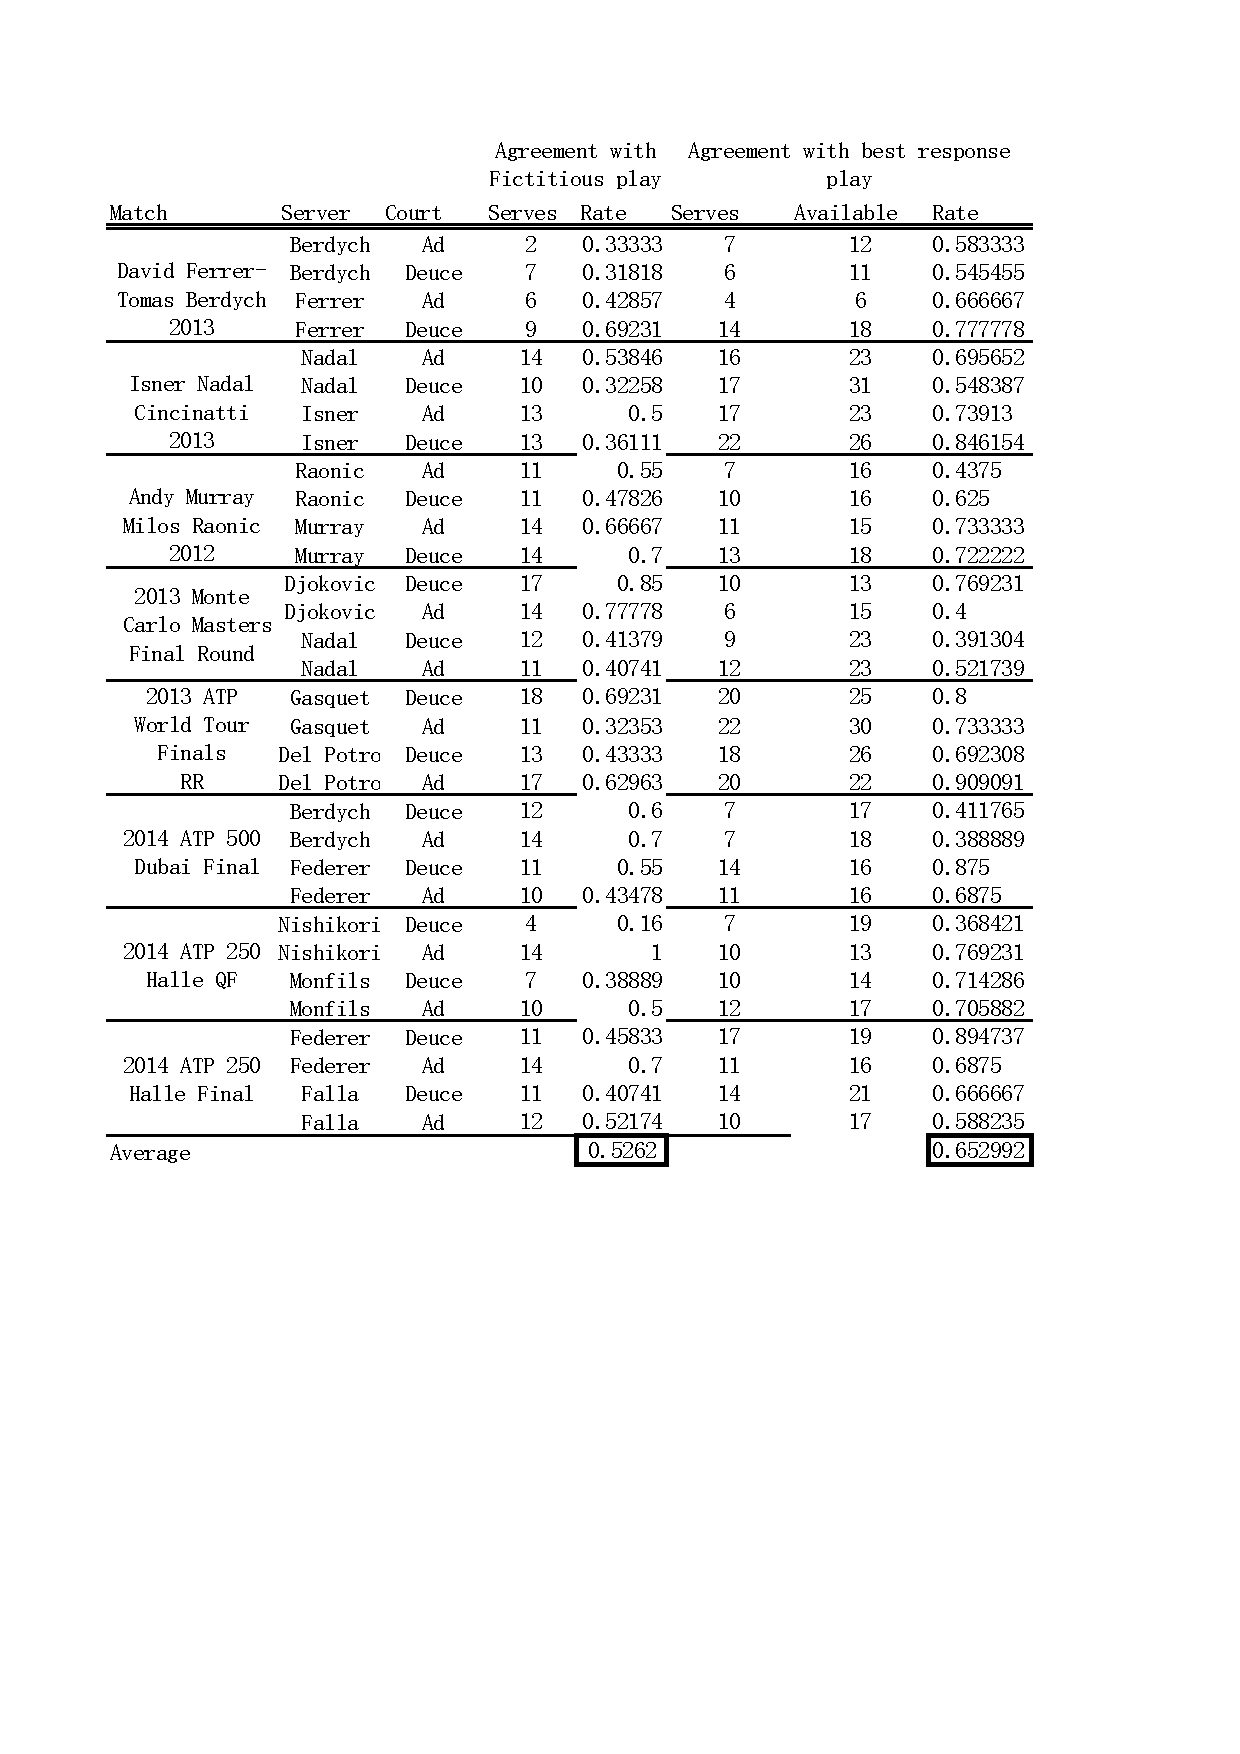
\includepdf{fictitious.pdf}


\bibliography{bibliography}{}
\bibliographystyle{alpha}

\end{document}
